\documentclass[conference]{IEEEtran}
\usepackage{times}

% numbers option provides compact numerical references in the text. 

\usepackage{graphics} % for pdf, bitmapped graphics files
\usepackage{epsfig} % for postscript graphics files
%\usepackage{mathptmx}
%\usepackage{newtxtext}
%\usepackage{newtxmath}
\usepackage{times} % assumes new font selection scheme installed
\usepackage{amsmath} % assumes amsmath package installed
\usepackage{amssymb}  % assumes amsmath package installed
%\usepackage{amsthm}
\usepackage{mathtools}
\usepackage{bm}
\usepackage{mathrsfs}
\usepackage{xcolor}
\usepackage{cite}
\usepackage{threeparttable}
\usepackage{multirow}
\usepackage{bigdelim}
\usepackage{algorithm}
\usepackage{algorithmicx}
\usepackage{algpseudocode}
\usepackage{graphicx}
\usepackage{subfigure}
\usepackage{comment}
\usepackage{pifont}

\usepackage{amsmath}

\usepackage[numbers]{natbib}
\usepackage{multicol}
\usepackage[bookmarks=true]{hyperref}

%\pdfinfo{
%  /Author (Homer Simpson)
%   /Title  (Robots: Our new overlords)
%  /CreationDate (D:20101201120000)
%   /Subject (Robots)
%   /Keywords (Robots;Overlords)
%}

\begin{document}


%\title{Theoretically Complete Solution to the Optimal Non-repetitive Coverage Task of Arbitrary Shape Object with Minimal Discontinuities for a Non-redundant Robot Manipulator}
\title{An Improved Maximal Continuity Graph Solver for Non-repetitive Manipulator Coverage Path Planning (TBC) \textcolor{red}{I don't think we can call it optimal, I feel we don't know it is the optimal one! just more efficient!}}%: Graph Separation and Rejoining}
% <ty> If we use ``rejoining" then we need to change all ``combining" to ``rejoining"
% other alternatives:
% Maximal Continuity of a Planar Dual Graph for Optimal Manipulator Coverarge
% Optimal Manipulator Coverarge as Maximal Continuity of a Planar Dual Graph
% Yue Wang suggested that the algorithm may be used in other problems that also use dual graph. So I didn't mention "coverage" or "manipulator"

%
%\author{Tong Yang, Jaime Valls Miro, Yue Wang and Rong Xiong
%\thanks{$^1$ Tong Yang, Yue Wang and Rong Xiong are with the State Key 
%Laboratory of Industrial Control and Technology, Zhejiang University, P.R. China. 
%}
%\thanks{$^2$ Jaime Valls Miro is with the Centre for Autonomous Systems (CAS), University of Technology Sydney (UTS), Sydney, Australia.}
%\thanks{$^*$ Corresponding Author. \newline \indent
%E-mail address: {\tt\small wangyue@iipc.zju.edu.cn}}
%}

\maketitle

\begin{abstract}
\begin{comment}
The non-repetitive coverage tasks carried out by manipulators have been widly involved in industrial applications. Due to the non-linearity of the manipulator kinematic, the end-effector would inevitably be lifted off the surface of the object. 
Existing results modelled the problem into a painting problem of a planar dual graph, and proved that all optimal solutions can be collected in finite steps, where the physical meaning of the optimality is the minimality of the number of end-effector lift-offs. 
Although the algorithm can terminate in finite iterations, the algorithmic complexity is too large to be applicable to complicated graphs. Concretely, for a graph with $M$ cells and $N$ edges, and denote by $\alpha_i$ the number of adjacent cells of the $i$-th cell and $K_i$ the number of possible colours to fill in the cell, the complexity is enumerating all possible colours of each cell and all edges,  
$\prod_{i = 1}^M K_i^{\max\{\alpha_i-2, 1\}}\cdot 2^N$, where $N \gg M$ is indicated by Euler's formula. 
In this work, with the aim to avoid enumerating all topolgoical edges, we notice a topological invariance when solving the graph, the number of intersections of colours. Keeping/removing edges is essentially equivalent to enumerating different solutions of removing an intersection.  
Then, we propose a novel graph separation strategy such that each sub-graph is guaranteed to be intersection-free. Through solving sub-graphs individually and combining them to form the optimal solutions, we reduce the complexity to $\prod_{i = 1}^M K_i^{\max\{\alpha_i-2, 1\}}$, i.e., directly removing the multiplication of the term $2^N$. 
\end{comment}
A provable computational improvement to the problem of maximal continuity during non-repetitive object coverage with non-redundant manipulators is proposed in this work, where the physical meaning of optimality translates to minimal number of end-effector lift-offs. Existing solutions enumerate each point on the surface with multiple ``colours'' according to the joint-configuration adopted, and model the problem as a painting problem of a planar dual graph with $M$ topological cells (a fully-connected section of end-effector points that can be painted with the same set of possible colours) and $N$ topological edges
(indicating the different choices of colour available). 
% (indicating the possible different choices of colour). 
% or, we can say indicating the difference between coverable colours. 
These works have proven that all optimal solutions can be collected in a finite number of steps. However, the solution grows exponentially in the size of $N$, becoming potentially intractable even for relatively simple graphs.
%\textcolor{blue}{However, with enumerating all edges being an unavoidable step, a term $2^N$ must appear in the algorithmic complexity of the algorithm. }
The proposed solution aims to avoid the need to enumerate all %topological 
the edges by exploiting a topological invariance in the number of colour intersections. It has been observed that keeping/removing edges is equivalent  \textcolor{red}{to enumerating  solutions where colouring intersect (see note in .tex, I feel this needs to stand out more clearly)}
% note: I am ok on how it is written, it is however not yet clear to me how we do this, so unsure if the explanation is fully correct, as not very descriptive, lacks punch - I leave until I read further into the paper, hope it gets clea. 
A novel graph separation strategy is thus proposed such that each sub-graph is guaranteed to be intersection-free. By solving sub-graphs individually and combining them to form the set of all optimal solutions, the complexity is proven to be reduced by a factor of $2^N$. Challenging scenarios are presented to validate the computational advantage of the proposed strategy.
\end{abstract}

\IEEEpeerreviewmaketitle

\section{Introduction and Related Work}
The problem is motivated by the non-revisiting coverage path planning (NCPP) along the surface of an object with a non-redundant manipulator. 
Given the object's surface, the manipulator, 
the surrounding obstacles in the workcell and their related poses, for each reachable point on the surface there exist a finite number of inverse kinematic solutions in the manipulator configuration space. 
% Here we only focus on the coverable part in the surface. 
Disregarding singular configurations~\cite{Yoshikawa1990Translational}, the collection of all valid configurations form disjoint sets in joint-space. When the manipulator transits from one set to another, it adopts a new pose altogether whereby the end-effector cannot remain on the object, being forcibly detached from the surface. This is an undersirable effect for tasks where smoothness and continuity are critical such as painting, deburring, welding, etc. 
In these instances, the desired solution translates to designing manipulator trajectories such that the end-effector visits each point on the surface exactly one time, whilst ensuring a minimum number of transition between joint-space sets, or lift-offs. 

\begin{comment}
To simplify the description, we assume that the coverable area of each colour is simply-connected.  \textcolor{red}{I believe this is not just an assumption, but a requirement: does the proposed solution holds for non-simply connected? I don't think so, in which case we should say this differently, pls confirm}. 
% Here it has been generalized to the constraints of ``simply-connected cells", the same as Tmech work. As we have no page go into detail formulae of the cost calculation, we no long need further simplication on the global connectivity of colours.
% <jvm> 
\end{comment}

\begin{figure}[t]
\centering
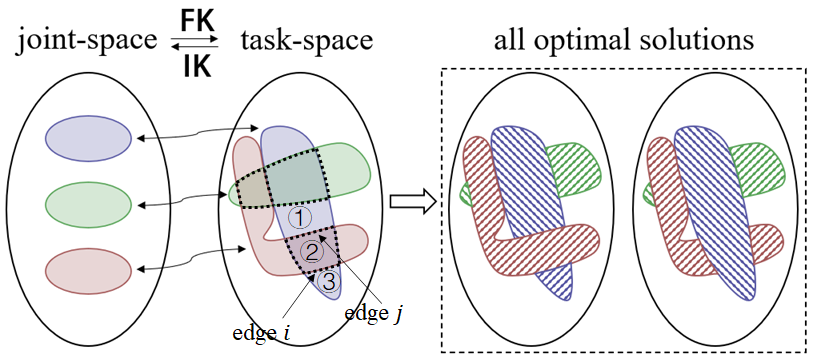
\includegraphics[width = 0.44\textwidth]{figures/mapping_2}
\caption{A toy illustration of the problem arising when planning optimal non-revisiting coverage paths with a manipulator: valid robot configurations form disjoint sets in joint-space, while their task-space FK mapping images (end-effector poses) may overlap. 
%, which is the key problem to be solved for non-repetitive CPP task. 
In the example, which for simplicity is illustrated with cells that are maximally $2$-overlapped, the resulting task-space graph 
% we don't really show the full graph, but will get complex, so we show snippets. I think clear like this.
%\textcolor{blue}{It is the initial graph (in the ``task-space" ellipse), and the right two graphs are the only } 
conveys $N = 11$ undetermined edges constructed as shown by the dashed lines, thus separating the graph into $M = 11$ cells.
To facilitate the understanding whilst limiting clutter in the graph, 3 cells and 2 edges ($i$ and $j$ in dashed blue-green and blue-red respesctively) are singled out.
Solving the NCPP problem for the set of edges in the example can easily reveal all the optimal solutions in this case (two, depicted), demarcating the minimal bound for lift-offs as four. 
%\textcolor{red}{Tong, make sure this is 100\% correct; would a solid green split the solution into more lift-offs? we won't say, I want to say the above, but but pls make sure. No need to explain it to me, I just want a "Yes it is correct" answer, I can feel it to be the case, but have not expand the graph fully to be 100\% sure}.
%<ty> Yes, it is correct. 
It is easy to appreciate how as more colours ``intersect", the algorithmic complexity to find the optimal solutions will soon escalate (more intricate examples are provided in Section~\ref{section_experiment}). 
%note: can we lead here in the txt with a final comment where intuitively hint at the proposed solution by means of exploiting the topological 'intersections'? not sure we can do so clearly with this example, if you can, add a succint note here in that regard. Otherwise we simply present the problem of how complexity grows
It is also intuitive that should the green colour remain a complete set, both the red and blue colour cells would be split into further disconnected parts, leading to extra lift-offs. %so in order to get global optimality, the green colour must be sacrificed. 
This hints at the fact ``intersecting" colours %may be a \textit{topological invariance} of the graph that 
can be exploited to reduce the complexity of the solution.
}
\label{fig:mapping}
\end{figure}


%\subsection{Existing Solutions Revisiting}
% <ty> we may again propose the result in Tmech. See how many pages can be left for this. 

% \textcolor{red}{We should open up in more generic fashion, describing a wider range of alternatives in a small paragraph, then note the best, ours, as below}.

%\begin{color}{blue} See whether this paragraph perfectly covers the content of the next paragraph (citation will be added tomorrow, save time to modify algorithms) \end{color} 

Early reports on the generic \textit{coverage path planning} (CPP) problem focused on geometric path designing, particularly for mobile platforms operating in planar surfaces, such as boustrophedon~\cite{} or spiral paths~\cite{}. 
Additional strategies were later proposed that transformed the coverable region into smaller partitions, or \textit{cells}, where continuous coverage paths could be guaranteed. A body of novel partioning \textit{cellular decomposition} strategies emerged~\cite{}~\cite{}, applied directly onto the area to be covered. This is an ineffective strategy when transfered from task to joint space for manipulator planning since the kinematic mapping between the two spaces is non-bijective: as illustrated in Fig.~\ref{fig:mapping}, the forward kinematic relationship from the configuration space to the surface is surjective (many-to-one) and locally flat (one-to-one from each connected component of the valid configuration space to the surface). 
%See Fig.\ref{fig:mapping} for an illustration of the kinematic mapping. 
The problem is further compounded when the end-effector can only visit each point on task-space once, leading to numerous pose reconfigurations during the motion of the end effector~\cite{}.
%extended the results to more complex scenarios, providing a complete solution~\cite{}. 
%leading to significant gains towards overall smoothness in the resulting manipulator paths~\cite{}. 
%A body of novel partioning \textit{cellular decomposition} strategies extended the results to more complex scenarios, providing a complete solution~\cite{}~\cite{}. 
%This is an adequate constraint for mobile robot navigation assignments for instance~\cite{}, but does not translate well for manipulator CPP tasks~\cite{} operating in joint-space, not in the task-space, 
\textcolor{red}{I feel still no refs to other works for manipulator and NCPP-like, very limited refs - can we borrow more from RSS20 and ICRA21 and add here, before we talk about ours?}
Recent propositions in the literature decomposed the task-space area into a %initial 
topological graph ensuring continuous joint-space coverage within each cell, and looked for solutions where maximal continuity between cells existed~\cite{Yang2020Cellular}, as intuitively depicted in Fig.~\ref{fig:mapping}. \textcolor{red}{our other works too? maybe too much as NO other CPP manip. refs!} All maximal-continuous cellular decompositions were proven to be collectable in a finite number of steps, defined by edges which represent the smallest, inseparable elements and cells that could only have a finite number of different sub-divisions.  

%\textcolor{red}{ Recent propositions in the literature formulate a solution in two stages, an initial optimal cellular decomposition at its core, which can then be followed by an arbitrary coverage path planning routine (\textcolor{red}{ref boust., or spiral, ...)} within each cell~\cite{Yang2020Cellular}. As a result, the problem is thus transformed into an optimal matching of each point on the surface to one of its IK solutions under a continuity constraint. Representing different sets of joint-space configurations as different colours, a point on the surface can be painted with multiple colours (see Fig.\ref{fig:mapping}). The cell, a region of task-space contiguous points, is defined as a maximal connected region in which all points can be painted with same set of possible colours.} 

%\textcolor{red}{Point 1: trying to make the case of what we are trying to do and why: justification! not just describing the how, but the why!} 
This is however an intense computational process, growing exponentially in the size of the graph. Let there be $M$ topological cells and $N$ topological edges in the modelled graph to be solved. The number of edges for the $i$-th cell is $\alpha_i$, and denote the number of possible colours to fill cell $i$ ($K_i$).   
It has been shown how a binary array of length $\alpha_i$ can be used to index all possible different divisions of cell $i$~\cite{Yang2020Cellular}, whereby 
%$0$ at the $r$-th position enforcing the cell having different color to its $r$-th adjacent cell, while $1$ enforcing a same choice of colour. 
$0$ at a given position enforces the cell having a different color to its adjacent cell, whilst $1$ compels the same choice of colour. An example of this is illustrated in \ref{fig:many_to_one} for the edge solution $1111$ and 2 possible colours available for painting. \textcolor{red}{we don't show what the adjacent colours in the example are, so does this matter? would it be the same for 0000, or 0001 ...? don't provide a long explanation to me pls, try to think like a reade who has NEVER seen [1], and finds this all of a sudden. We are trying to use it to explain the complexity of the problem, and how to improve it. Nothing more. Would he get this from reading this explanation and Fig 1? not sure. We need Fig 1 to explain the complexity issue below, it MUST stay, and I like the caption. But from the drawing and the explanation, I don't think the reader can relate this to the earlier Fig 1, where the problem is clearly defined and teh concept of cell and topological edge also I believe is clearly estated and defined).}
The enumeration of a single cell is executed on all cells to find all optimal solutions.
\textcolor{blue}{This note is for which definition? }\textcolor{red}{??? ``The enumeration of a single cell is executed on all cells'' : this unncessary enumeration is the key to our proposed improvement, but from that single sentence droped out of context is not possible to see - what is the problem here? you make a statement, mathematically correct, but why that is a problem is not expressed. You need to "lead", explain with common language, not just drop things like these ...}
%\textcolor{red}{Since every two adjacent cells share a same edge, the overall number of elements to be enumerated is the number of internal edges (the edges on the boundary of the coverable area cannot be ``connected"). For simplicity, we approximately say it is ``all edges", which makes no difference to the contribution of this work because the term containing $N$ will be totally removed in this paper. --- you can't say this, makes not sense, if it makes no contribution and ``will be removed'', whay is it there in the first place!!??}
While this has been proven a finite exercise~\cite{Yang2020Cellular}, it comes at a significant cost. Since every edge has two adjacent cells, 
the relation of $\alpha_i$ to $N$ is established by
\begin{equation}
N = \frac{1}{2}(\sum\limits_{i=1}^M \alpha_i - \tilde{N})
\end{equation}
($\tilde{N}$ simply denotes the number of edges on the outer boundary of the graph, %(with adjacent cells $-1$ ) 
which are determined and thus need not be enumerated). 
%Note that, although proving the finiteness of dividing each cell into sub-cells is enough for proving the finiteness of the whole process, the overall algorithmic complexity is far more than $2^N$, 
It has been shown in the Fig.~\ref{fig:many_to_one} counterexample how there is no one-to-one correspondence between the edge and painting solutions. 
The edge solution depicted, 1111, could be painted with 4 different valid painting alternatives.
Generically \textcolor{red}{is this from Tmech? I think so, so we need to reference it, not just drop it expecting the reader will be able to figure that out, not possible!} it has been proven by the cell sub-divion strategy described in~~\cite{Yang2020Cellular} how if $\alpha_i \geq 4$, cell $i$ will be iteratively divided into $(\alpha_i-2)$ $3$-edge sub-cells\footnote{Here for simplicity we only consider the worst case presented in~\cite{Yang2020Cellular}. Beyond dividing fully into $3$-edge cells, the complexity of enumerating other cell sub-divisions is omitted \textcolor{red}{but it is also part of the enumeration of edges, shouldn't we? or you mean that taking the worst case, 4 adjacent cells, represents the highest computation and therefore we only need to conseder this case for complexity calculation? - which I agree with}.}, and each sub-cell can be individually assigned with $K_i$ colours. Let there be $E_i$ different ways to divide cell $i$ into sub-cells, the overall complexity %\footnote{Here we disregard speeding-up tricks proposed in existing literature, because they are also valid in the algorithm proposed in this work. } 
can then be calculated as
\begin{equation}\label{equ:tmech_complexity}
\prod\limits_{i=1\atop\alpha_i \geq 4}^{M}E_i\cdot \prod\limits_{i = 1}^M K_i^{\max\{\alpha_i-2, 1\}} \cdot 2^N
\end{equation}
%<ty> We have to explicitly consider $E_i$, or else the algorithm may be false. It is too late to change all subsequent figures and equations today, and I will do it tomorrow. 
%\textcolor{red}{see .tex comment}
% <jvm> I feel we can cut this out and will have no impact on the paper - once we change title and abstract ref to dual-graph. If you agree, we do:
% <ty> OK. 
\begin{comment}
Also note that as a dual graph of the commonsense ``node-edge" graph, the cells, edges and vertices correspond to the nodes, edges and faces (temporarily denoted as $F$ which has no usage in the NCPP problem), respectively. Then the relation of the number of cells $M$ and the edges $N$ is given by the Euler's formula for planar graph, 
\begin{equation}
N-M = F-2
\end{equation}
In a complicated graph we must have $F\gg 2$, then $N \gg M$. 
\end{comment}
\begin{comment}
\begin{color}{blue}
We observe that enumerating an edge is a too trivial process to lead to different topologies of the resulting solution. See Fig.\ref{fig:mapping}, where if edge $i$ is kept, then $j$ need not be removed, because even if cell \ding{172} and \ding{173} are connected, it makes no difference to the topology if cell \ding{174} is not connected together. 
In other words, existing works have avoided equivalent cellular decompositions under the equivalence of continuous modification of the cutting paths of cells. But looking at the topology of resulting solution from a top-down view might further avoid carrying out equivalent multi-step processes in enumerative solving. 
In this paper, we introduce a high-level abstraction of the topology, the \textit{intersection}, which is the origin of the multiplicity of the optimal solutions. We show that intersections are unavoidable and have to be enumeratively solved. 
However, through separating the graph into intersection-free sub-graphs, all intersections are implicitly enumerated while sub-graphs are combined. As a result, the algorithmic complexity of enumerating all edges, $2^N$, is removed. 
%\textcolor{red}{Point 2: the above chunk, between point 1 and 2, needs to be more succintly described, to be revised, too late now. I like the maths, will stay, but it is hard to read an focus on what matters: solution it is complex, we provide a more efficient way to solve it, quantify it, and prove the improvement. An algorithm solution is proposed to capitalise on the topological invariance} 
\end{color}
\end{comment}

Careful examination of the topological graph leads in this work to the introduction of a high-level abstraction, the \textit{topologcal  intersection} which is the origin of the multiplicity of the optimal solutions. It is hereby proven that intersections are indeed unavoidable and have to be enumeratively solved. However, separating the graph into intersection-free sub-graphs, leads to all intersections being implicitly enumerated while \textcolor{red}{when??} the sub-graphs are recombined later to calculate the final solution. The end result is the removal of the substantial complexity in enumerating all edges, $2^N$. 


\begin{figure}[t]
\centering
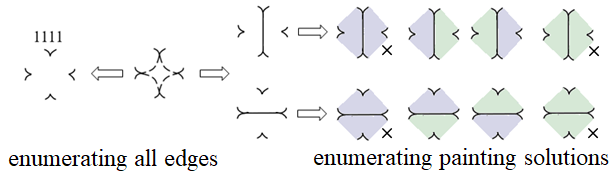
\includegraphics[width = 0.48\textwidth]{figures/many_to_one_2}
\caption{Let a cell with $4$ adjacent cells (a $4$-edge cell) have 2 possible colours ``blue" and ``green", then $\alpha = 4, K = 2$. From the point of view of solving edges, the binary number $1111$ specifies one solution, but the corresponding valid painting solutions are multiple, $4$ to be precise: there are $E=2$ ways to divide the multi-edge cell into $3$-edge sub-cells, and $\alpha-2 = 2$ sub-cells are generated which can be filled withe the $K (=2)$ possible colours. After enumerating $E\cdot K^{\max\{\alpha-2, 1\}}$ cases, four of them are removed (no subdivision when there is only one possibly colour for all sub-cells), shown crossed-out, leaving the remaining four valid painting solutions.}
\label{fig:many_to_one}
\end{figure}

The remainder of this paper is organised as follows. Section~\ref{section_intersection} introduces the concept of \textit{topological intersection} and shows its vital role to solve simple graphs. Section~\ref{section_graph_separation} justify a divide-and-conquer approach separating more complex graph into sub-graphs. Solutions to these can then be combined to construct the optimal solutions for the full graph as described in Section~\ref{section_full_graph}. Details  about the complexity advantage in solving the problem following the proposed strategy is mathematically proven in Section~\ref{section_complexity}, whilst experimental results from simulations are collected in Section~\ref{section_experiment}. Final concluding remarks are gathered in Section~\ref{section_conclusion}.

\subsubsection*{Notation}
\textcolor{red}{Not critical!ok as is. But pls make sure this clarification is absolutely necessary. If use sparingly later, or can be noted when first used, maybe best than here. Otherwise it is fine, we have bigger problems!} 
The word \textit{divide} refers to the division of a cell with a \textit{cutting path}, whilst a graph is \textit{separated} into multiple sub-graphs through a \textit{separating path}. Thus, \textit{cells being separated} means a graph is separated via dividing the specified cells into parts, then one sub-cell is connected to one sub-graph while the other sub-cell is connected to another sub-graph.  The variables $i,j$ and $n$ are used for indexing. 

\section{Optimality via ``Topological Intersections''}
\label{section_intersection}
In this section we introduce a topological invariant variable, \textit{intersection}. 
The concept of intersection is revealed through proposing a \textit{divide-and-conquer} solution to a kind of simple graphs, maximally $2$-overlapped graphs, where the intersections are easy to figure out. 
\subsection{Definition of Intersections}
\begin{figure}[t]
\centering
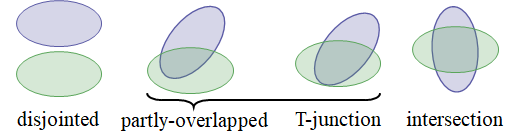
\includegraphics[width = 0.4\textwidth]{figures/basic_shape_2}
\caption{Illustration of basic relations between the reachable area of two colours. T-junction is a special case of the partly-overlapped distribution of colours, while it can be transformed back to a normal case through continuously modifying the boundary of colours.  }\label{fig:basic_shape}
\end{figure}
\textcolor{blue}{See whether we can find a better sentence about ``intersection is what"}
In a special definition, an intersection is a kind of overlapping between coverable region of two colours. 
In a generic definition, the intersection describes an inevitable interruption of the connectivity of one colour by other colours. 
The coverable area of two colours may be fully disjointed, partly overlapped or intersected, as shown in Fig.\ref{fig:basic_shape}. 
The two colours can both keep connected in the disjointed and partly overlapped cases, but in the intersection case, one colour being connected will make the other colour being truncated into two parts. 
And obviously, either colour being connected is an optimal solution. In a complicated graph, such an intersection may introduce two set of optimal solutions, in one set all solutions keep one colour connected, while in the other set the other colour is connected. 


\begin{figure}[t]
\centering
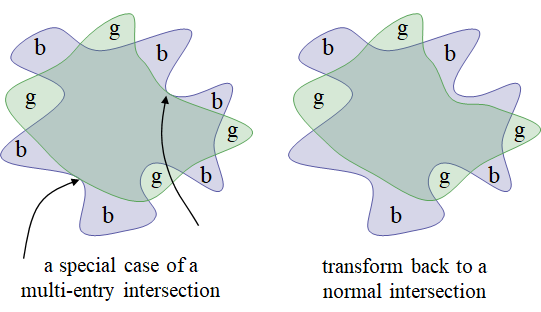
\includegraphics[width = 0.35\textwidth]{figures/multi_entry}
\caption{An intersection with $8$ entries. For some special cases that two consecutive adjacent cells can be filled in same colour, through shrinking the boundary of colour, it can be transformed back to the normal case. }\label{fig:multi_entry}
\end{figure}
Seeing the intersection in Fig.\ref{fig:basic_shape} as of $4$ entries, the intersection with arbitrary number of entries is intuitive, as shown in Fig.\ref{fig:multi_entry}. After simplifying the intersection by merging consecutive adjacent cells which have same set of possible colours, the intersection will have $n$ (an even number) entries. 
It is observed that, for each adjacent cell (say the $i$-th, labelled cyclicly), if it is connected to any other adjacent cell through the intersection, then the $(i-1)$-th and $(i+1)$-th cell cannot be connected. 
I.e., once we connect two entries through solving the intersection, another pair of entries are impossible to be connected. 
So the minimal number of continuous regions for an $n$-entry intersection is $\frac{n}{2}+1$. 


However, note that even if the optimal number is directly deduced, we still have to enumeratively solving the intersection to get all optimal cellular decompositions. 
\begin{comment}
Denote the cyclic sequence of adjacent cells of an $n$-entry intersection by 
\begin{equation}
\mbox{intersection}_n = [g_1 b_1 \cdots g_i b_i \cdots g_{\frac{n}{2}} b_{\frac{n}{2}}]
\end{equation}
where ``b" and ``g" represent colour ``blue" and ``green", the iterative enumeration can be represented as 
\begin{equation}
\begin{aligned}
\mbox{solution}_n =& \{[g_1 b_1 \cdots g_i b_i \cdots g_{\frac{n}{2}} b_{\frac{n}{2}}]\}\\
=& \{[g_1 b_1 \cdots b_{i-1}(g_i) b_i \cdots g_{\frac{n}{2}} b_{\frac{n}{2}}]\}\\
&\cup \{[g_1 b_1 \cdots b_{i-1})g_i( b_i \cdots g_{\frac{n}{2}} b_{\frac{n}{2}}]\}\\
=& \{g_i, [g_1b_1\cdots g_{i-1}b_{\{i-1, i\}}g_i\cdots g_{\frac{n}{2}}b_{\frac{n}{2}}]\}\\
&\bigcup\limits_{j \neq i} 
\end{aligned}
\end{equation}
where $(\cdot)$ represents dis-connectivity of elements. 
\end{comment}
For the $i$-th entry, we will separately consider (a) connecting it to other entries, or (b) keeping itself disconnected so that the $(i-1)$-th and $(i+1)$-th entry can be connected. Both of them go to optimal cellular decompositions. 

\subsection{Solution of Maximally $2$-overlapped Graph}
\textcolor{red}{note: is this provided for illustration only with a smaller problem? we then move on to the width-2 strip sub-graphing, that is the actual final solution. Correct? If so, we should intro this differently. }
\textcolor{blue}{Yes, the divide-and-conquer strategy cannot be used when there is no $1$-colour cell to separate. We just use it to show that intersections are unavoidable and we have to proactively solve them. (and in the next section we will show that, when separating graph through multi-colour cells, the ``solving" of intersections has to be ``enumeration". )
} 

\begin{figure}[t]
\centering
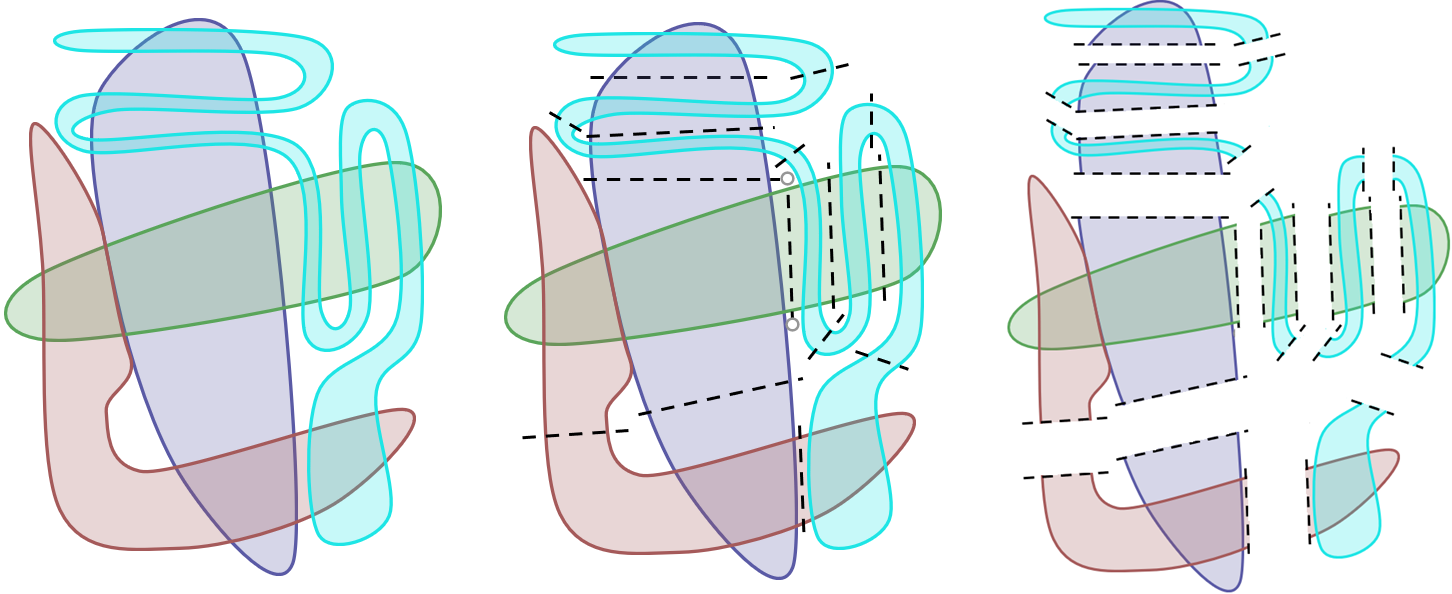
\includegraphics[width=0.44\textwidth]{figures/two_overlapped_graph}
\caption{The graph is separated into $9$ sub-graphs through $1$-colour cells, shown in dashed line. The number of continuous regions is $4+3\times 8 = 28$ and we created $15$ dashed lines, so the number of continuous regions in the original graph is $28-15=13$, i.e., $12$ lift-offs are necessary to finish this coverage task. However, for all optimal cellular decompositions, each intersection has to be enumerated. The total number of optimal cellular decompositions will be $2^8 = 256$, and no any two of them are equivalent under continuous modification of cell boundaries. }\label{fig:two_overlapped_graph}
\end{figure}

Here we provide an efficient \textit{divide-and-conquer} solution to the maximally $2$-overlapped graphs (for each cell, there are at most $2$ possible colours). 
The efficiency of the solution is intrinsic to the uniqueness of colour of the cell to be separated. 
A case is given in Fig.\ref{fig:two_overlapped_graph}. 
The key step is to separate the graph into sub-graphs through dividing $1$-colour cells connecting intersections. 
The dashed lines are the places where we separate the original graph into sub-graphs. Since the divided cell only has unique coverable colour, we divide one cell into two unconnectable cells (belonging to different sub-graphs), so the number of continuous regions of the graph should be the sum of continuous regions in sub-graphs and minus the number of dashed lines. 
Moreover, we can arbitrarily combine the optimal solutions of sub-graphs to form optimal solution of the original graph. 
However, even if the computational cost of combining solutions of sub-graphs has been reduced, no intersection was removed. All intersections are solved in sub-graphs, and all optimal solutions are collected through full combination of different optimal solutions of intersections. 

\subsection{Local Property of Intersections}
In Fig.\ref{fig:two_overlapped_graph} there exist two parallel colours which are simultaneously crossed by the third colour. Then the graph cannot be trivially separated, because the multi-colour cells are adjacent, with no $1$-colour cell in between. 
In fact, the intersection and the parallelness are trouble makers in clarifying topology between different colours. Generalized cases of the intersection between two sets of parallel colours are used for later discussion and are shown in Fig.\ref{fig:non_optimal_subgraph} and Fig.\ref{fig:local_in_other_graph}. 
The crucial observation of parallelness and intersection is that they describe local distribution of colours but not a global characteristic between colours: Two colours can be intersected in a part of the graph, while be parallel at another part of the graph. 
With more colours involved, such as the case shown in Fig.\ref{fig:three_overlapped_graph}, intersections are highly coupled, so that we cannot even figure out intersections. Only what we know is that, the number of intersections in the partly-solved graph will not reduce under continuous modification of cell cutting paths, thus all intersections are implicitly reduced when all edges and all cell colours are enumerated (in existing methods~\cite{Yang2020Cellular}). 

\begin{figure}[t]
\centering
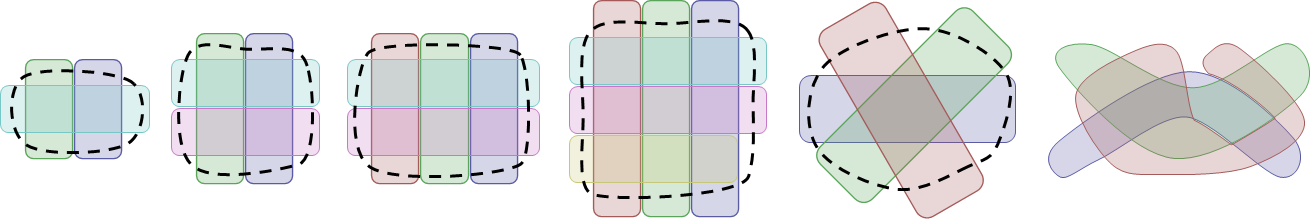
\includegraphics[width = 0.48\textwidth]{figures/three_overlapped_graph_2}
\caption{Some demo graphs with intersections. 
The dashed circle marks a part of the graph which contains intersections. 
From left to right: special cases of $2$-overlapped intersection constructed by $2\&1$ parallel colours, $2\&2$ parallel colours, $2\&3$ parallel colours and a further special case of $3\&3$ parallel colours (where whether the orange colour intersects with the blue colour is closely related to the optimal solutions. Now they only form a T-junction), a normal $3$-overlapped intersections and a complicated $3$-overlapped graph which we cannot even figure out where is the intersection given too many intersections and parallelness of colours in it. }\label{fig:three_overlapped_graph}
\end{figure}

%In this section, we introduced a topological invariance of an unsolved graph, intersections. 
%An efficient solution of maximally $2$-overlapped graph is proposed to reveal the significant role of intersections in solving a generic graph. 
%The number of intersections is shown invariant under homeomorphic modification of cellular decompositions while a valid cellular decomposition is free of intersection, so all intersections have to be iteratively solved. 
%In the next section we will show that intersections cannot be solved locally, then the process to remove an intersection has to be ``enumeration all cases". 
%However, such efficient solution cannot be generalized to arbitrary graph separation, as separating graph through multi-colour cells cannot be arbitrarily combined. the key step to improve the efficiency is to address the redundant steps of enumerating intersections, which is the main focus of the next section. 



\section{Separating Graph into Width-$2$ Strips}
\label{section_graph_separation}
We observe that for an intersection-free graph, the list of colour choice of all boundary cells uniquely characterise the solution of the graph. 
This motivates us to find a novel topological structure called \textit{width-$2$ strip}, or \textit{strip}, which is proven intersection-free. 
With the graph being separated into strips and each strip being solved individually, we combine all solutions of strips to generate all solutions of the original graph, where all optimal solutions are included. 
\textcolor{blue}{We might put this sentence to conclusion of this section: 
Recall that intersections are intrinsic to the graph, non-existence of intersections in strips means that all intersections are automatically solved while strips are combined, which do not add extra algorithmic complexity. 
}

To avoid redundant discussion caused by $E_i$ in (\ref{equ:tmech_complexity}), we assume that all $n(\geq 4)$-edge cells have been divided into $3$-edge sub-cells before applying this algorithm. 

\subsection{Motivation: Property of Intersection-Free Graphs}

Let there be $\tilde{N}$ edges on the boundary of a graph which is assumed free of intersection, denoted as $\{e_i|i = 1, \cdots, \tilde{N}\}$. Each $e_i$ has only one adjacent cell, denoted as $c_i$, which has $K_i$ possible colours. 
For an $n(\geq 4)$-edge cell, it may have multiple edges exposed to the boundary of the cell, but we have assumed that it has been fully divided into sub-cells, so each edge is only adjacent to one sub-cell whose colour is well-defined, so we don't make further clarification.  
For simple description, we say \textit{the colour of $e_i$} is the colour of the (sub-)cell adjacent to $e_i$.  
Then, we can use a string to represent the colour of edges in order, called the \textit{characteristic string} of the graph. 

A crucial observation of an intersection-free graph is that, the connectivity of the graph can be uniquely characterised by the colour on the boundary, or more precisely, the cyclic list of colour, $[e_1, \cdots, e_{\tilde{N}}]$. 
% <ty> Can I use the sub-graph in the experiment section for illustration? Or use another demo? 
To verify this, let the colour of all boundary edges be determined. See Fig.\ref{} for illustration. Picking up any two edges with same colour, we must be able to judge their connectivity through this graph. If the connectivity is undetermined, that means we may find another pair of edges whose connection may prevent these two edges being connected. However, this is the intersection, which contradicts our assumption of the intersection-free property of the graph. 

\begin{figure}[t]
\centering
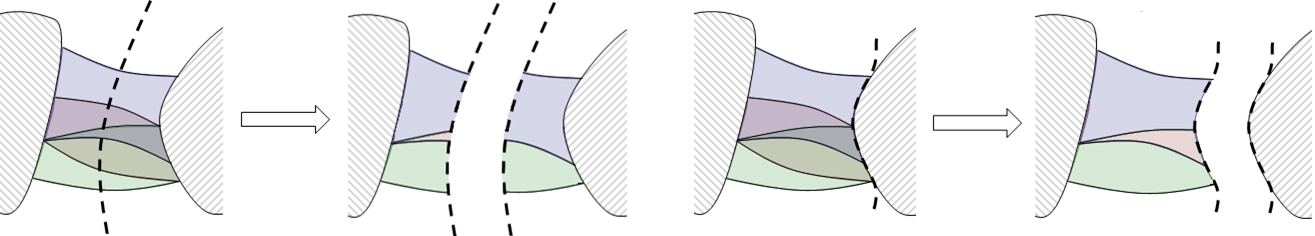
\includegraphics[width=0.48\textwidth]{figures/separation_at_edges_2}
\caption{If a graph is separated through division of multi-colour cells, the constraint of the cell vanishes, then in the sub-graphs there may exist solutions that after being combined is non-optimal, such as the case given in left. If the graph is separated along edges, we will not incur such problem. }\label{fig:separation_at_edges}
\end{figure}


\subsection{Relation between Optimality of Graph and Its Sub-Graphs}
Before we go into relations between graph and sub-graphs, we have to claim a basic criteria for separating a graph into sub-graphs. 
Different from separating the graph through an $1$-colour cell, where the solutions of sub-graphs can be arbitrarily combined, if we separate the graph through multi-colour cells, as illustrated in Fig.\ref{fig:separation_at_edges}, the constraints of the original cell vanishes, then proven non-optimal solutions may appear. In contrast, separating the graph through existing edges has the same effort, which is desired. 
So in sequel our graph separation process should  follow existing edges in the graph, which makes Fig.\ref{fig:non_optimal_subgraph} and Fig.\ref{fig:local_in_other_graph} reasonable. 

%It is also observed that if the edge has multi-colour adjacent cells, then the combination of different solutions of sub-graphs will have non-trivial cost variation (not $-1$ as used in Fig.\ref{fig:two_overlapped_graph}). 

\begin{figure}[t]
\centering
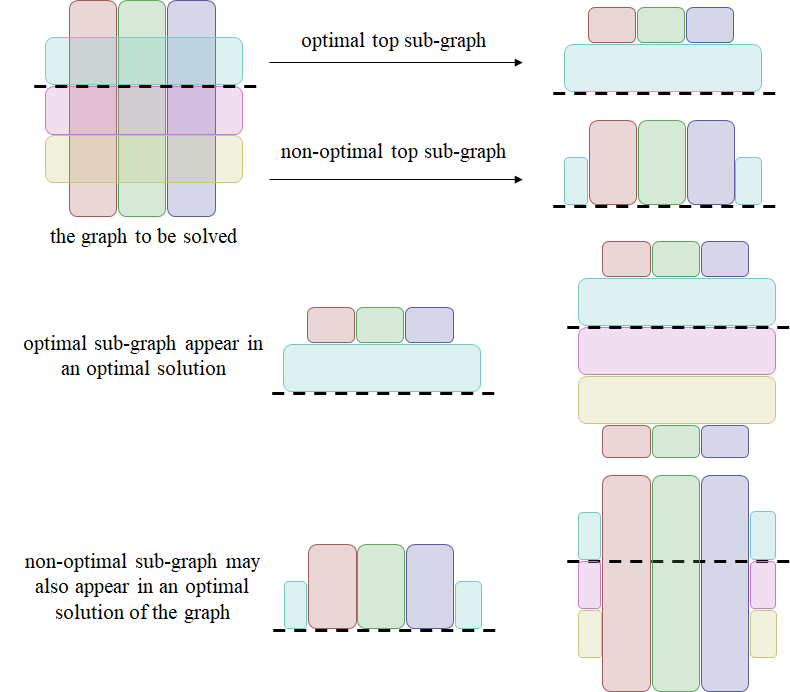
\includegraphics[width=0.44\textwidth]{figures/local}
\caption{Separating the graph through the dashed line, we show the optimal solution and a non-optimal solution of the sub-graph. It is noticeable that both of them form optimal solutions of the original graph. }\label{fig:non_optimal_subgraph}
\end{figure}

\begin{figure}[t]
\centering
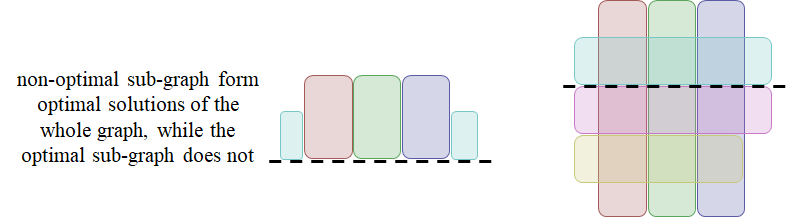
\includegraphics[width=0.44\textwidth]{figures/local_in_other_graph}
\caption{Another graph to be solved which has the same sub-graph as the case shown in Fig.\ref{fig:non_optimal_subgraph}. The optimal solution consists of only the non-optimal sub-graph but not the optimal sub-graph. }\label{fig:local_in_other_graph}
\end{figure}


Then, we claim that there is no guarantee about the global optimality of combining optimal solutions of sub-graphs. In other words, when a graph is separated into sub-graphs, we have to collect all solutions of each sub-graph. (It is not a bad thing if all solutions of sub-graphs can be enumerated, since in this case solving sub-graphs is unnecessary. )
This is proved by two examples illustrated in Fig.\ref{fig:non_optimal_subgraph} and Fig.\ref{fig:local_in_other_graph}. In \ref{fig:non_optimal_subgraph} both optimal and non-optimal solution of the sub-graph will form an optimal solution of the original graph. And in Fig.\ref{fig:local_in_other_graph} it is shown that non-optimal sub-graph is included in optimal solution of the original graph while the optimal sub-graph is not. 
%See Fig.\ref{fig:non_optimal_subgraph}, where the graph to be solved is an intersection between three parallel colours and another three parallel colours. The optimal solution is obviously either connecting all horizontal colours or connecting all vertical colours. 
%We can see from this case that optimality of the sub-graph is not equivalent to the optimality of the whole graph. So if a graph is separated into sub-graphs, we should store all solutions of sub-graphs but not only optimal solutions. 
%Another problem is that the optimality of a solution of the sub-graph hugely depends on other sub-graphs. A case is given in Fig.\ref{fig:local_in_other_graph}. 
%So we can only judge the optimality after we pick one solution from each sub-graph and combine them to form a solution of the whole graph. 
%In other words, in the absense of arbitrary combination of the solutions of sub-graphs, the algorithmic complexity of the graph is the multiplication but not the sum of the complexity of solving each sub-graph. 

\begin{figure*}[t]
\centering
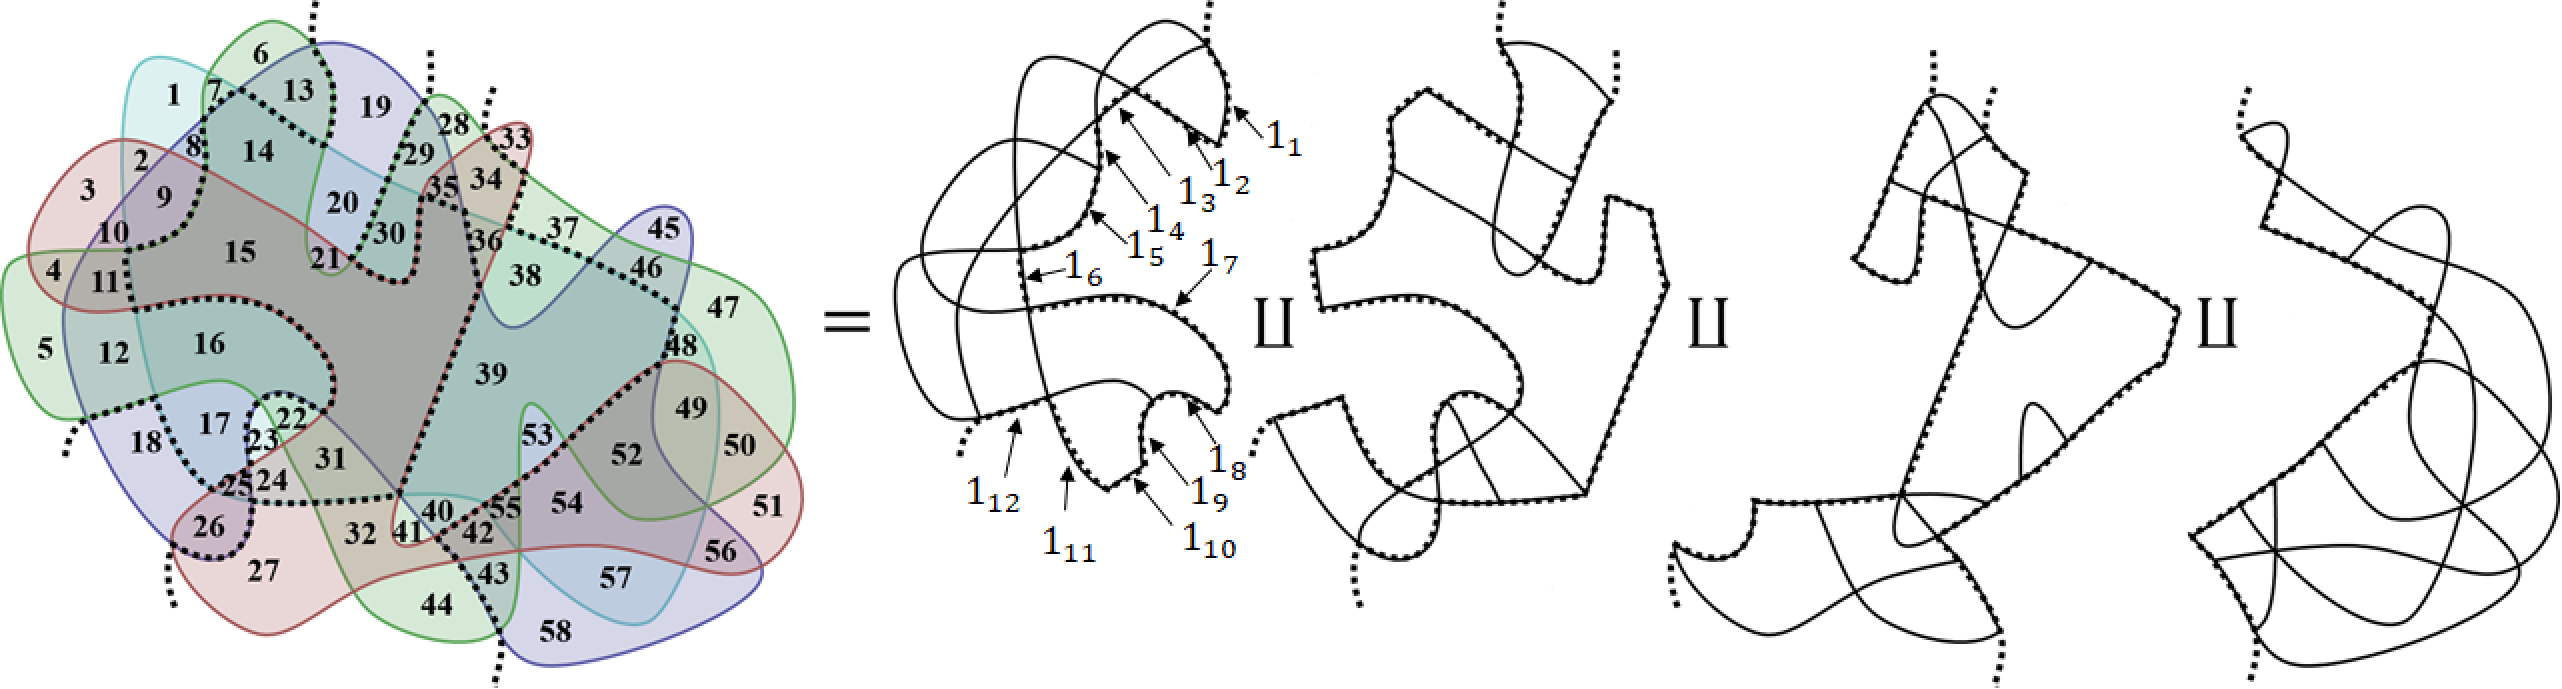
\includegraphics[width=0.96\textwidth]{figures/complicated_graph/graph_separation_with_index}
\caption{\textcolor{blue}{TODO: divide some multi-edge cell into triangles as is done in experiment. }A demo graph with $4$ colours and $58$ cells. The coproduct sign $\coprod$ means that collecting all solutions of different sub-graphs are totally independent. It is easy to verify that there is impossible to form any intersection in each sub-graph. Then, the boundary characteristic uniquely corresponds to a cellular decomposition of the sub-graph. Note that the graph separation is not unique, and we only need a valid one. }\label{fig:complicated_graph}
\end{figure*}

\begin{figure*}[t]
\centering
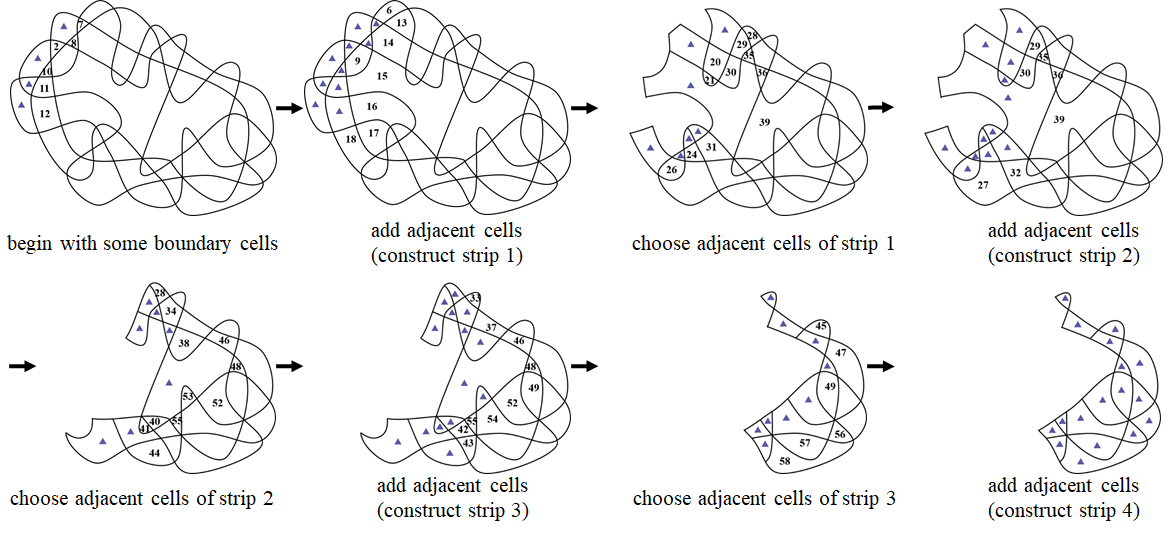
\includegraphics[width=0.96\textwidth]{figures/complicated_graph/steps}
\caption{The concrete steps to separate the graph given in Fig.\ref{fig:complicated_graph} into intersection-free strips. }\label{fig:steps}
\end{figure*}



\subsection{Definition of Width-$2$ Strip}
Note that in the following subsections, we assume that multi-colour cells have been divided into sub-cells, such that if there still exists multi-colour cells, it is inseparable and must be filled in with a single colour. An illustration of the graph containing inseparable multi-edge cells is given in Fig.\ref{fig:complicated_graph} and Fig.\ref{fig:steps}, while a worst-case demo is given in Fig.\ref{fig:hat}. 

We observe that, when an intersection appears in a part of the graph, there must exist at least $4$ entries. 
The intersection may not be fully described in a single multi-colour cell (shown in Fig.\ref{fig:three_overlapped_graph}, where intersection of parallel colours also exist). 
And the entry may not be a single edge (shown in Fig.\ref{fig:three_overlapped_graph}, the simple intersection formed by three colours can be seen as of $6$ entries but has $12$ edges).  
Given too many variants of the intersections, we may consider its opposite: If in each sub-graph, each cell only has at most $3$ adjacent cells, then there is impossible to be an intersection. 
To this aim, we define \textit{width-$2$ strip} as a sub-graph in which all cells have at most $3$ adjacent cells. 
It is named after its construction which is given in the next subsection. 

For the $i$-th strip, let there be $\beta_i$ edges in the boundary of the strip, its \textit{characteristic string} is represented by a list of $\beta_j$ colours, recording the colour of the edges in order. 
% Haven't dicided which demo graph we will use here, so leave it now. 
For example, 




\subsection{Separating Graph into Width-$2$ Strips}
The discussion is given on a complicated example shown in Fig.\ref{fig:complicated_graph}, which is computationally unaffordable if we enumerate all edges and cells. Following our assumptions, we assume that all multi-edge cells have been divided before starting graph separation. 
We first select several boundary cells of the graph (cell $1, 3, 4, 5$ in this example) and regard them as elements of strip $1$.
% <ty> I'm not sure whether you can understand the below, and whether it is necessary. 
\begin{comment} 
We appropriately select the initial cells for the first strip, such that there is no multiply-connected strips constructed which introduce unnecessary discussion. A counter-example in this case is choosing all boundary cells, $1, 6, 19, 28, \cdots, 4, 3$. 
It is easy to create valid separations, so we omit further discussion on the initial selection. 
\end{comment}
The cells are only selected at the boundary, so it can be seen of width $1$. 
Then, for each adjancet cell of the sub-graph, we check whether accommodating the cell into the sub-graph will violate the constraint of maximal $3$ adjacent cells. If not, then it is added to the sub-graph. 
For example, after we have added cell $2, 8, 9, 10$ to strip $1$, cell $9$ has three neighbours, thus cell $15$ cannot be inserted to strip $1$. 
After inserting extra cells, strip $1$ is constructed. 
Only another one ``column" of cells are expected to be added to the strip, so we call the strip as width-$2$ strip. 
For $\alpha(\geq 4)$ edges, then $\alpha-3$ edges must be exposed to the boundary of the strip, which will be separately considered when we calculate the algorithmic complexity. 

\textcolor{blue}{Stop here. A lot below can be removed if we use this ``motivation". }

To avoid introducing extra discussion when combining sub-graphs, we enforce all adjacent cells of strip $1$ being selected into strip $2$, so that strip $i$ will only have common boundary with strip $(i-1)$ and $(i+1)$. 
Then adjacent cells of strip $2$ are iteratively checked to be included. 
Iteratively putting the adjacent cells of the previous strip into the current strip and adding more cells satisfying the constraint of maximally $3$ adjacent cells in a single sub-graph, the whole graph is finally separated into width-$2$ strips. 


\subsection{Solving Sub-Graphs}
Since the strip is free of intersections, given same solution of boundary cells, all solutions of other cells are topological equivalent. 
In other words, if a cell do not have edge exposed to the boundary and it has same colour as its adjacent cells, then it must fill in with the same colour. So we may freely use one solution to represent all the solutions having same colours on the boundary.  
So the complexity of finding all different solutions is no more than the multiplicity of the number of possible colours of the boundary cells. 
In the example shown in Fig.\ref{fig:complicated_graph}, for strip $1$, there are $12$ edges connecting to strip $2$, whose adjacent cells are $13, 13, 7, 8, 9, 11, 16, 16, 17, 17, 17, 12$. 
Using previous notation, the number of possible colours of these cells are denoted as $K_{13}, K_{13}, K_{7}, \cdots, K_{12}$. Then there are at most $K_{13}^2K_{7}\cdots K_{17}^3K_{12}$ different solutions to fill in colours to this strip. 

\begin{color}{blue}
In particularly, the edges in strips need not be enumerated. As long as we fill in the adjacent cells, the existence of the edge is automatically judged. 
\end{color}

\section{Speeding-up Tricks}
\textcolor{red}{note: this is general to all sub-graph solutions to reduce enumerations. I put in its own section so it can be identified as , but it feels small? }
\textcolor{blue}{It is general. Through graph separation, the (sub-)graph has new property, ``intersection-free". So many tricks can be explored. I didn't give expanded discussion because we needn't them in computing algorithmic complexity. We can do them if we want better improvement (I'm thinking of it, to appear in this paper or the next one). }
Note that although the optimality of sub-graph solutions has no relation to the optimality of the whole graph, some global non-optimality and equivalences between different cellular decompositions can be easily judged in sub-graphs. 
Besides, since sub-graphs are strip-like, the cells are almost ``ordered", then some speeding-up tricks may appear and are open to consider. 
Here we just give an example of them. (We will not consider any tricks when calculating the algorithmic complexity in the next subsection): 
If a cell only have one edge exposed to the boundary of the sub-graph, and it is able to be covered jointly with its adjacent cells, then it must do so because of the equivalence between cellular decompositions. 
For example, after cell $13, 6, 7, 1, 8, 2$ are painted in enumerating all solutions of strip $1$ and we assume cell $2$ is in red and cell $8$ is in cyan, it comes to painting cell $9$. 
Cell $9$ can be covered using either red or cyan. However, if we enforce cell $9$ to be blue, then cell $10$ must also be in blue, or else cell $9$ has different colour to all its neighbours. Even if it may have same colour with cell $15$, we can continuously modify the boundary of the final cellular decomposition to ``shrink" cell $9$ into cell $15$, which is apparently equivalent. The constraint also works when we solving cell $11$, $16$, etc. 
Applying more constraints while enumerating solutions of strips, we will get significantly less number of solutions for each strip.  
\textcolor{red}{note: but is this a formalism that we use? you just talk about how you'd do for the example in Fig 10, how is that generalisable? what are these "constraints" that reduce the number of solutions? not sure I get it, if you can only say for the example, no good, should not be here. Maybe a small note on the "solving subgraphs" above, but even there, if not generic how to make it part of the algorithm? }

\section{Full Graph Solution}\label{section_full_graph}
After collecting all solutions of all strips, picking up one solution of each strip, we can combine them to form a solution of the original graph. 
The edges that used as separation lines are automatically solved through comparing the colour of its two adjacent cells which are in different sub-graphs. 

Whether keeping the edge or removing the edge automatically depends on the colour of its adjacent cells, and the cost variation is the same as~\cite{Yang2020Cellular}, whose physical meaning is the number of continuous regions in the painted part of the graph. 
Compared with seeing strips as two separated sub-graph, when combining them, if the adjacent cells of an edge have same colour, and the cells have not been connected by previous combining process, then the cost $-1$.  

We given an example of combining the strip $1$ and $2$ in Fig.\ref{fig:complicated_graph}. 
The list of adjacent cells of the common edges between strip $1$ and $2$ are 
\begin{equation}
\begin{aligned}
&[13, 13, 7,~~  8,~  9,~  11, 16, 16, 17, 17, 17, 12] \mbox{ and }\\
&[19, 14, 14, 14, 15, 15, 15, 22, 23, 25, 18, 18]
\end{aligned}
\end{equation}
If cell $13$ and cell $19$ are in same colour, then the cost of the combined graph is one less than the sum of cost of two strips. After that, if cell $13$ and cell $14$ are also in same colour, notice that in strip $2$ we must have connected cell $19$ and cell $14$, so we need not further reduce the cost. 
Once the original graph is re-constructed, we know the number of continuous regions in the solution. Then we can judge its optimality. Check all possible combinations of solutions of sub-graphs, we will get all optimal solutions. 

\section{Complexity}
\label{section_complexity}
The proposed algorithm has been shown to consist of three steps: graph separation, solving each strip individually and finally constructing all optimal solutions by combining the individual strip solutions. 
Separating the graph only requires checking on each cell for one time, and we only need one valid graph separation, so the complexity of this part is defined by $\Phi = O(M)$. 
\textcolor{red}{note: many of these formulae can be embedded in the txt to gain space}
Indexing the number of cells in strip $i$ by $i_1, \cdots, i_{r_i}$, the cells have $\alpha_{i_1}, \cdots, \alpha_{i_{r_i}}$ edges, and the number of their coverable colours are written as $K_{i_1}, \cdots, K_{i_{r_i}}$. 
Intentionally considering the sub-division of cell which has more than $3$ edges, the complexity of solving strip $i$ will be 
\begin{equation}
\Psi_i = \prod\limits_{j = 1}^{r_i} K_{i_j}^{\max\{\alpha_{i_j}-2, 1\}}
\end{equation}
Since enumerating solutions of different strips are totally independent, the complexity is just summed up but not muliplied. And note that $M = \sum r_i$, 
\begin{equation}
\begin{aligned}
\Psi = \sum \Psi_i = & \sum\limits_{i} \left(\prod\limits_{j = 1}^{r_i} K_{i_j}^{\max\{\alpha_{i_j}-2, 1\}}\right)\\
\ll&\prod\limits_{i}\left(\prod\limits_{j = 1}^{r_i} K_{i_j}^{\max\{\alpha_{i_j}-2, 1\}}\right)\\
=&\prod\limits_{j = 1}^M K_j^{\max\{\alpha_j -2, 1\}}
\end{aligned}
\end{equation}

For the final part of the algorithm, the complexity is extremely sensitive to the concrete separation of the graph. 
For example, in the previous cases shown in Fig.\ref{fig:complicated_graph}, if cell $17$ is put into strip $2$ but not strip $1$, the graph separation is still valid. But then there will not be a $K_{17}^3$ term in the number of solutions of strip $1$, which is replaced by a $K_{16}$. 

We argue that a fair approximation is that all cells are exposed to the boundary of strips, so all of them will add one length to the characteristic of the corresponding strip. 
In addition, for the cell with $\alpha(\geq 4)$ edges, they are estimated to have $\alpha-2$ edges exposed to the boundary of the strip. 
So the length of the characteristic of strip $i$ is 
\begin{equation}
\sum\limits_{j = 1}^{i_r} \max\{\alpha_{i_j}-2, 1\}
\end{equation}
for the $j$-th number, the corresponding cell has $K_{i_j}$ possible colours, so the number of all different characteristics is 
\begin{equation}
\prod\limits_{j = 1}^{i_r} K_{i_j}^{\max\{\alpha_{i_j}-2, 1\}}
\end{equation}
When combining solutions of different strips to form solutions of the original graph, the solutions are arbitrarily combined, so the algorithmic complexity is the multiplication of complexity of all strips, 
\begin{equation}
\Xi = \prod\limits_i \left(\prod\limits_{j = 1}^{i_r} K_{i_j}^{\max\{\alpha_{i_j}-2, 1\}}\right)
= \prod\limits_{j = 1}^M K_j^{\max\{\alpha_j-2, 1\}}
\end{equation}
The overall complexity of the proposed algorithm is the sum of $\Phi$, $\Psi$ and $\Xi$, 
\begin{equation}
\begin{aligned}
\Gamma =& M + \sum\limits_{i} \left(\prod\limits_{j = 1}^{r_i} K_{i_j}^{\max\{\alpha_{i_j}-2, 1\}}\right) + \prod\limits_{j = 1}^M K_j^{\max\{\alpha_j-2, 1\}}\\
\approx&  \prod\limits_{j = 1}^M K_j^{\max\{\alpha_j-2, 1\}}
\end{aligned}
\end{equation}
Compared to previous solution~\cite{Yang2020Cellular} whose algorithmic complexity is given in (\ref{equ:tmech_complexity}), we provide an exponential improvement in the order of $2^N$. 

\begin{figure*}[t]
\centering
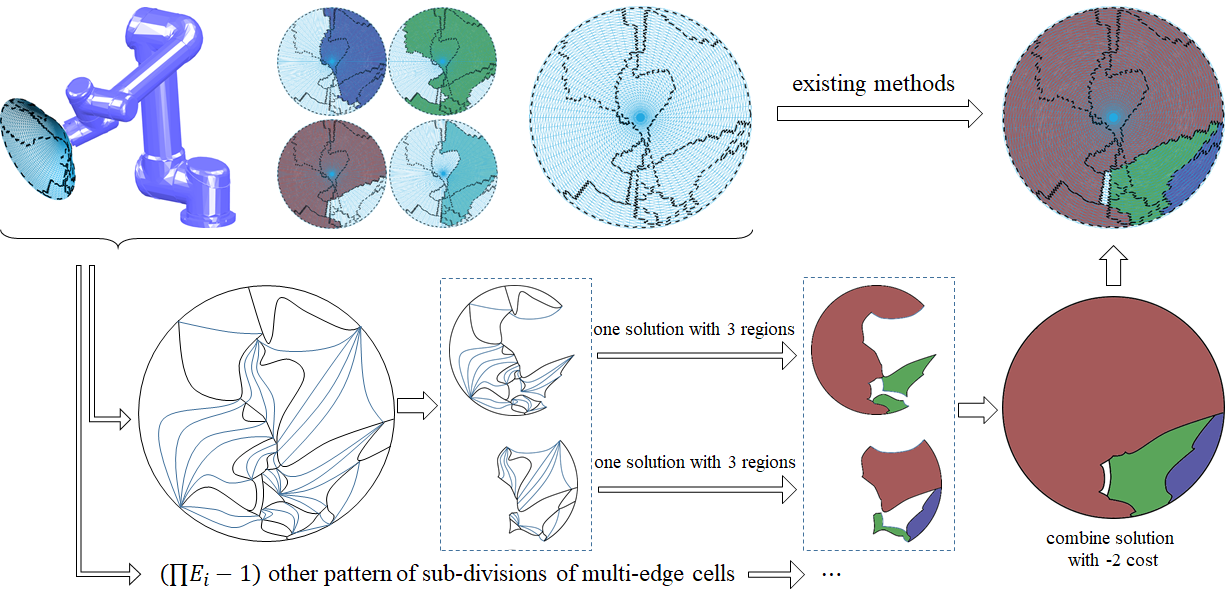
\includegraphics[width = 0.96\textwidth]{figures/hat_exp/fig_hat}
\caption{\textcolor{blue}{What if I directly use the sub-graph in this experiment to be the demo figures of the above algorithm section? }}\label{fig:hat}
\end{figure*}

\section{Experimental Results}\label{section_experiment}
\label{section_results}



% <ty> Suddenly I notice that the demo figure is not illustrative. Will change
An illustration of the iterative solving process of a hat-shape object is depicted in Fig.\ref{fig:hat}. 
Four continuous sets of manipulator configurations are represented in blue, red, green and cyan colour separately. 
Using existing algorithms~\cite{Yang2020Cellular}, the initial topological graph is directly enumerated. In solving an $\alpha(\geq 4)$-edge cell, the cell is divided into a set of $3$-edge cells. In naive enumeration we need to iteratively decide whether keep/remove each topological edges, and choose colour for each (sub-)cells, leading to complexity as (\ref{equ:tmech}). One of the graph after cell sub-divisions is shown in Fig.\ref{fig:hat}.  



\begin{comment}
Several representative simulation works have been implemented to validate the proposed algorithm on challenging  arbitrarily-shaped objects.
% the optimal non-revisiting coverage planning path is solved. 
Fig. \ref{fig_mobius_exp} presents the solution of polishing a Mobi\"{u}s strip, whose surface is non-orientable. The manipulator is required to maintain the EE normal to the surface for proper operation simulating a contact task such as polishing. This is rather challenging in this case 
since the strip is twisted, hence the orientation of the normal vector varies over the full $2\pi$ rads. However, the proposed algorithm 
is able to come up with an configuration mapping leading to an optimal solution where only $1$ lift-off is required over the entire object.

Fig. \ref{fig_ring_exp} depicts the process of covering the surface of a ``swimming'' ring, another closed surface with no boundary. 
This is a particularly challenging case, it can be seen how the topological graph is formed by cells which are all multiply-connected, 
yet the proposed algorithm is able to come up with an effective solution with a single configuration discontinuity to the NCPP problem. 

The examples in Fig.~\ref{fig:hill_multiply_conn}, Fig.~\ref{fig_hill_exp_0_10} and Fig.~\ref{fig_hill_exp_0_16} illustrate the solutions of covering a ``hilly terrain" with varying degrees of desirable manipulability~\cite{Yoshikawa1990Translational}. 
For a given configuration (colour) cell, the manipulability is explicitly depicted brighter for increasing manipulability for the given configuration. The threshold  varies from a minium of $0.06$ (Fig.~\ref{fig:hill_multiply_conn}) to at least $0.10$ (Fig.~\ref{fig_hill_exp_0_10}), up to at least $0.16$, the maximum where a solution can be found for the object (in Fig.~\ref{fig_hill_exp_0_16}).
As one would expect, a sharp reduction on the reachable area is observed as the manipulability tightens 
(mainly due to the limited mobility of the wrist-flipped configurations, shown in the bottom two configurations 
in Fig.~\ref{fig:manip_010_configs}), causing large fluctuations in the structure of the resulting cells and topology graphs. When the threshold goes to $0.16$, most of the kinematic-valid wrist-unflipped configurations are no longer valid, as depicted in Fig.~\ref{fig_hill_exp_0_16}. 
\end{comment}

\section{Conclusion}
\label{section_conclusion}


%% Use plainnat to work nicely with natbib. 

%\newpage 

\bibliographystyle{plainnat}
\bibliography{faster_solution_RSS21}

\end{document}


